\usetikzlibrary{arrows.meta}
\begin{frame}{HTTP proxies (1)}
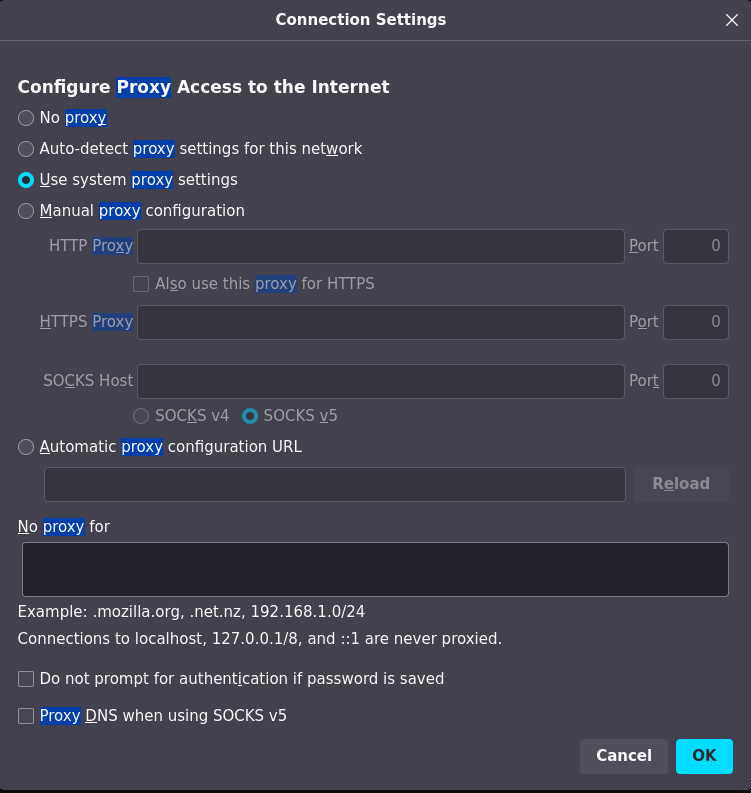
\includegraphics[height=0.9\textheight]{../http/moz-proxy-config}
\end{frame}

\begin{frame}
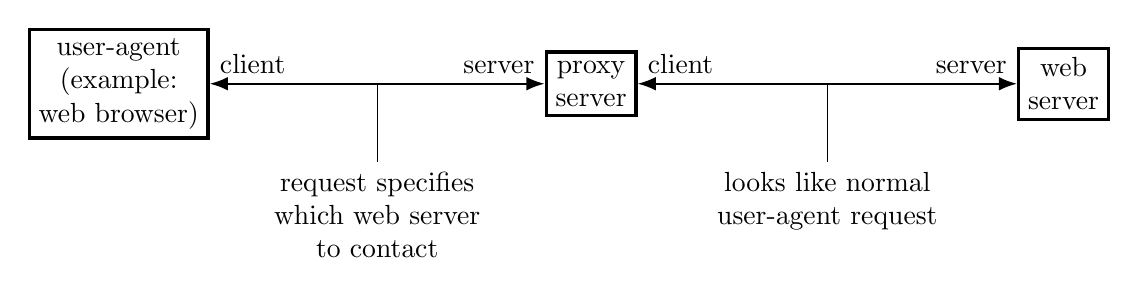
\begin{tikzpicture}
\node[draw, very thick,align=center] (user agent) at (0, 0) {
    user-agent \\ (example: \\ web browser)
};
\node[draw, very thick,align=center] (proxy) at (6, 0) {
    proxy \\server
};
\node[draw, very thick,align=center] (web server) at (12, 0) {
    web \\server
};
\draw[thick,Latex-Latex] (user agent) -- (proxy)
    node[pos=0,above right] {client}
    node[pos=1,above left] {server}
    coordinate[midway] (midpt cp);
\draw[thick,Latex-Latex] (proxy) -- (web server)
    node[pos=0,above right] {client}
    node[pos=1,above left] {server}
    coordinate[midway] (midpt ps);
\draw (midpt cp) -- ++(0cm, -1cm) node[below,align=center] {
    request specifies \\
    which web server \\
    to contact
};
\draw (midpt ps) -- ++(0cm, -1cm) node[below,align=center] {
    looks like normal \\
    user-agent request 
};
\end{tikzpicture}
\end{frame}

\begin{frame}[fragile]{HTTP proxies (2)}
browser$\rightarrow$HTTP(S) proxy sever: \\
\begin{Verbatim}
GET http://example.com/somesite HTTP/1.1
Host: example.com
...
\end{Verbatim}
\rule{.9\textwidth}{1mm}
\begin{itemize}
    \item instead of path, can put full URL
    \item doesn't have to be \texttt{http} URL
\end{itemize}
\end{frame}

\begin{frame}{proxy functionality}
    \begin{itemize}
    \item caching for multiple users
        \begin{itemize}
        \item reason for \texttt{Cache-Control: private}
        \end{itemize}
    \item filtering content
        \begin{itemize}
        \item antimalware, adblocking, etc.
        \end{itemize}
    \item logging content (example: debugging webapp)
    \item \ldots
    \end{itemize}
\end{frame}

\begin{frame}
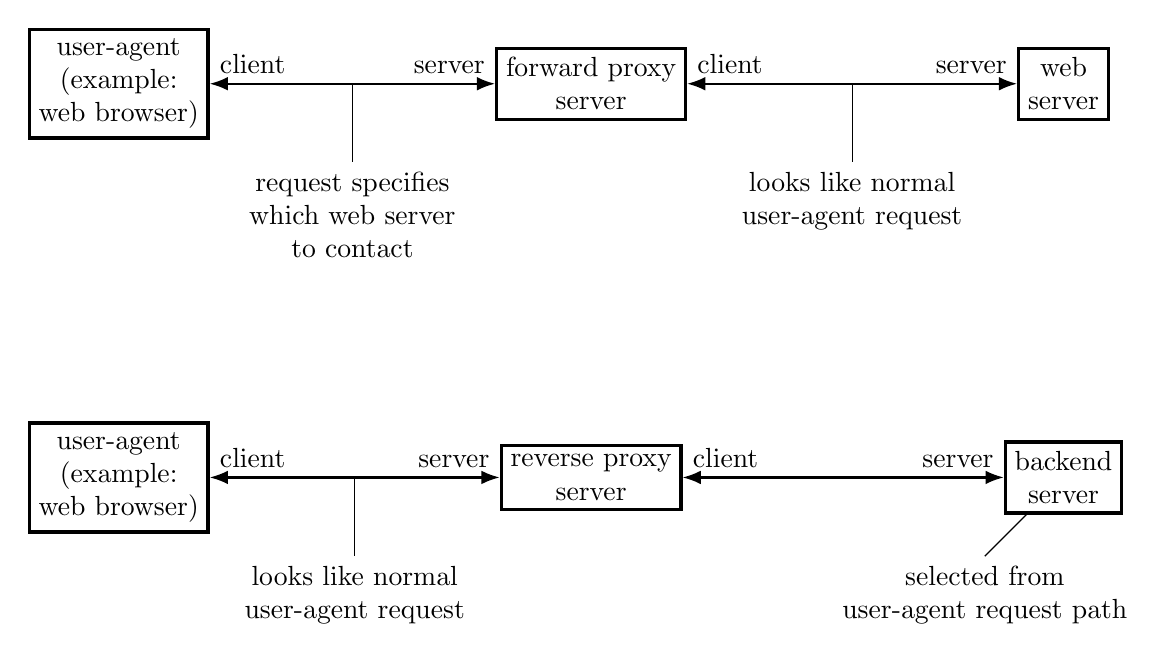
\begin{tikzpicture}
\node[draw, very thick,align=center] (user agent) at (0, 0) {
    user-agent \\ (example: \\ web browser)
};
\node[draw, very thick,align=center] (proxy) at (6, 0) {
    forward proxy \\server
};
\node[draw, very thick,align=center] (web server) at (12, 0) {
    web \\server
};
\draw[thick,Latex-Latex] (user agent) -- (proxy)
    node[pos=0,above right] {client}
    node[pos=1,above left] {server}
    coordinate[midway] (midpt cp);
\draw[thick,Latex-Latex] (proxy) -- (web server)
    node[pos=0,above right] {client}
    node[pos=1,above left] {server}
    coordinate[midway] (midpt ps);
\draw (midpt cp) -- ++(0cm, -1cm) node[below,align=center] {
    request specifies \\
    which web server \\
    to contact
};
\draw (midpt ps) -- ++(0cm, -1cm) node[below,align=center] {
    looks like normal \\
    user-agent request 
};

\begin{scope}[yshift=-5cm,name prefix=rvs-]
\node[draw, very thick,align=center] (user agent) at (0, 0) {
    user-agent \\ (example: \\ web browser)
};
\node[draw, very thick,align=center] (proxy) at (6, 0) {
    reverse proxy \\server
};
\node[draw, very thick,align=center] (web server) at (12, 0) {
    backend\\server
};
\draw[thick,Latex-Latex] (user agent) -- (proxy)
    node[pos=0,above right] {client}
    node[pos=1,above left] {server}
    coordinate[midway] (midpt cp);
\draw[thick,Latex-Latex] (proxy) -- (web server)
    node[pos=0,above right] {client}
    node[pos=1,above left] {server}
    coordinate[midway] (midpt ps);
\draw (midpt cp) -- ++(0cm, -1cm) node[below,align=center] {
    looks like normal \\
    user-agent request
};
\draw (web server) -- ++(-1cm, -1cm) node[below,align=center] {
    selected from \\
    user-agent request path
};
\end{scope}
\end{tikzpicture}
\end{frame}

\begin{frame}{reverse proxy}
    \begin{itemize}
    \item why not just go directly to actual web server?
    \vspace{.5cm}
    \item make multiple web severs appear as one? example:
        \begin{itemize}
        \item https://example.com/foo/XXX goes to https://foo-backend.example.com/XXX
        \item https://example.com/bar/XXX goes to https://bar-backend.example.com/XXX
        \item https://example.com/ goes to https://frontpage.example.com/
        \end{itemize}
    \item do caching, filtering, or similar on behalf of webservers
    \item split requests between multiple identical servers for performance
    \end{itemize}
\end{frame}
